% Created 2025-04-10 Thu 11:48
% Intended LaTeX compiler: pdflatex
\documentclass[11pt]{article}
\usepackage[utf8]{inputenc}
\usepackage[T1]{fontenc}
\usepackage{graphicx}
\usepackage{longtable}
\usepackage{wrapfig}
\usepackage{rotating}
\usepackage[normalem]{ulem}
\usepackage{amsmath}
\usepackage{amssymb}
\usepackage{capt-of}
\usepackage{hyperref}
\usepackage{minted}
\setlength{\parindent}{0em}
\author{Hankertrix}
\date{\today}
\title{MA0218 Mini Project: The Climate Forum}
\hypersetup{
 pdfauthor={Hankertrix},
 pdftitle={MA0218 Mini Project: The Climate Forum},
 pdfkeywords={},
 pdfsubject={},
 pdfcreator={Emacs 30.1 (Org mode 9.7.11)}, 
 pdflang={English}}
\begin{document}

\maketitle
\setcounter{tocdepth}{2}
\tableofcontents \clearpage\section{Preface}
\label{sec:org92c4e57}
The entirety of the project is contained within the \texttt{main.py} Python file,
and that also includes the slides.
The project makes use of \href{https://marimo.io/}{Marimo}, an alternative
to the Jupyter notebook format, and makes use of its slides.
Thus, \href{https://marimo.io/}{Marimo} is needed to display the slides and
run the notebook.
The data is also needed for the slides to display properly,
as the slides makes use of the data for its visualisations.
\section{Installing required software}
\label{sec:orgeeab832}

\subsection{Marimo}
\label{sec:orgbcc1fb6}
To install \href{https://marimo.io/}{Marimo} using \texttt{pip}, run the command below:

\begin{minted}[]{shell}
pip install marimo
\end{minted}

If you are using \href{https://www.anaconda.com/}{Anaconda},
run the command below to install \href{https://marimo.io/}{Marimo}:

\begin{minted}[]{shell}
conda install conda-forge::marimo
\end{minted}

\newpage
\subsection{Other required libraries}
\label{sec:org1ce1484}
The project also makes use of the libraries
covered in the lectures, such as:
\begin{itemize}
\item \href{https://numpy.org/}{Numpy}
\item \href{https://pandas.pydata.org/}{Pandas}
\item \href{https://matplotlib.org/}{Matplotlib}
\item \href{https://seaborn.pydata.org/}{Seaborn}
\item \href{https://scikit-learn.org/stable/}{Scikit-Learn}
\end{itemize}

If you are using a package manager like \texttt{pip}, \texttt{poetry}, \texttt{pdm} or \texttt{uv},
you can run the commands below to automatically install
the required packages.

\begin{itemize}
\item For \texttt{pip}:

\begin{minted}[]{shell}
pip install -r requirements.txt
\end{minted}

\item For \texttt{poetry}:

\begin{minted}[]{shell}
poetry install
\end{minted}

\item For \texttt{pdm}:

\begin{minted}[]{shell}
pdm install
\end{minted}

\item For \texttt{uv}:

\begin{minted}[]{shell}
uv install
\end{minted}
\end{itemize}

\newpage
\section{Running the notebook}
\label{sec:org56bfbb0}
To run the notebook, change to the directory
where you have downloaded the program,
making sure that the data file is also
in the same folder, and use the command below:
\begin{minted}[]{shell}
marimo run main.py
\end{minted}

\href{https://marimo.io/}{Marimo} should automatically open your browser,
similar to how Jupyter would, and you should be
able to view the notebook in the browser as slides.

\begin{center}
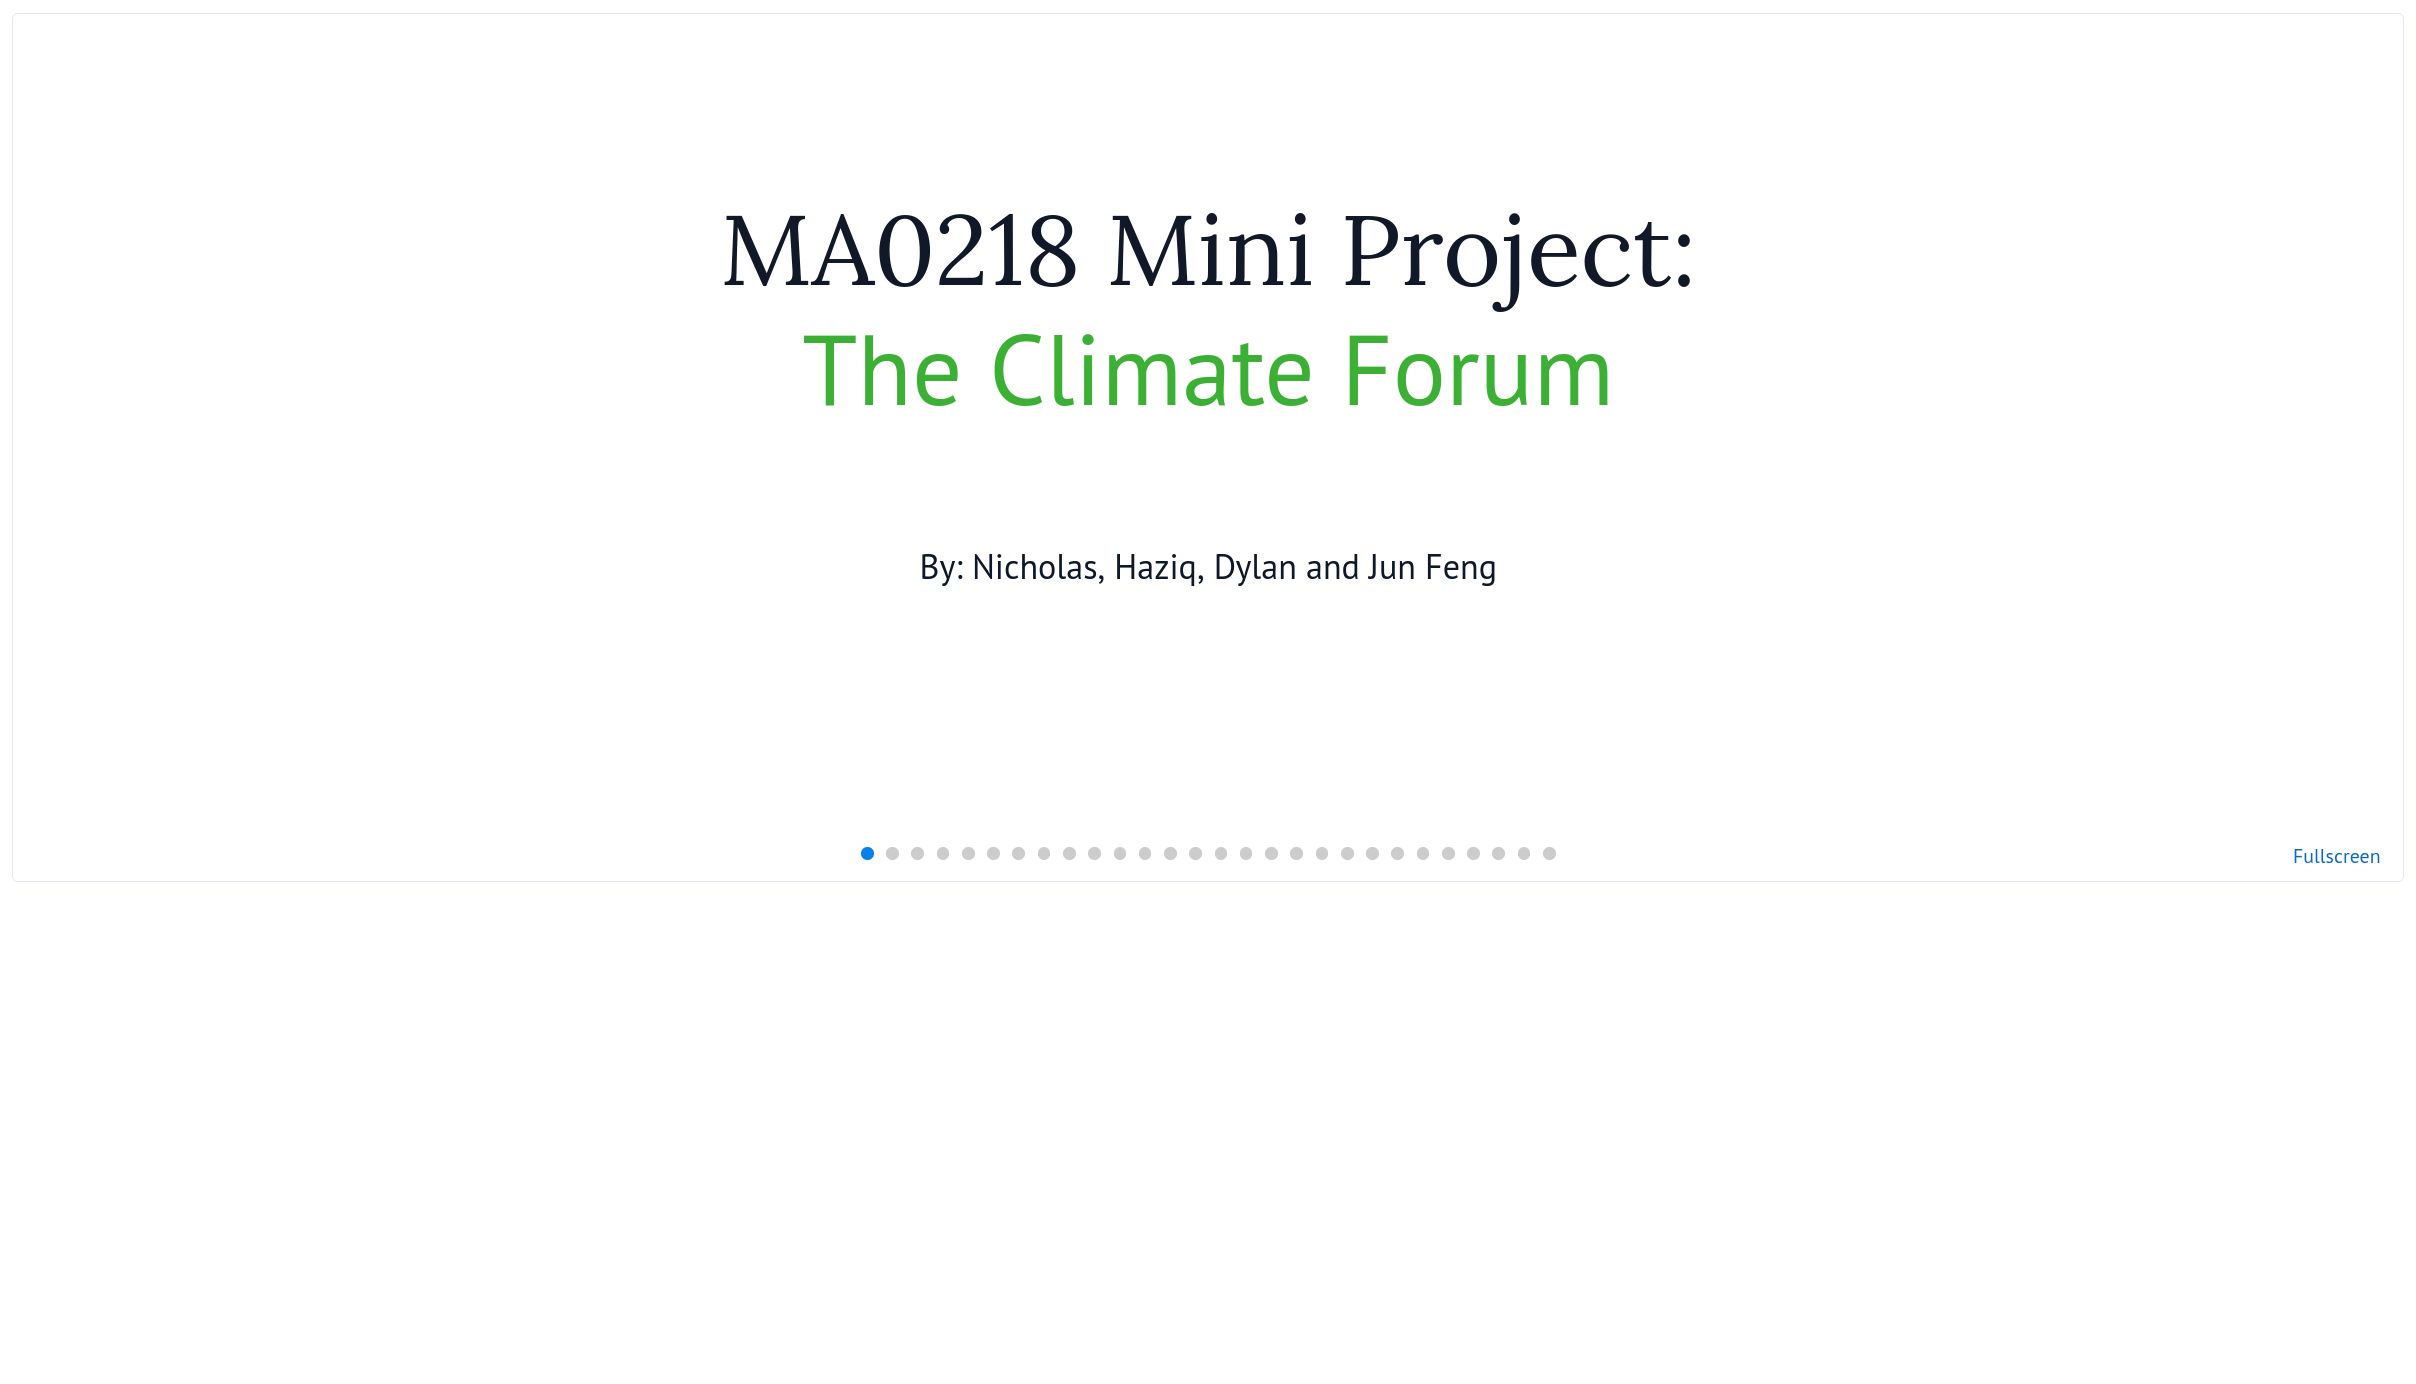
\includegraphics[height=15em]{./images/result-of-running-the-notebook.png}
\end{center}

If you would like to see the code, instead of running
the above command, use the command below to view it
in a notebook format:

\begin{minted}[]{shell}
marimo edit main.py
\end{minted}

\begin{center}
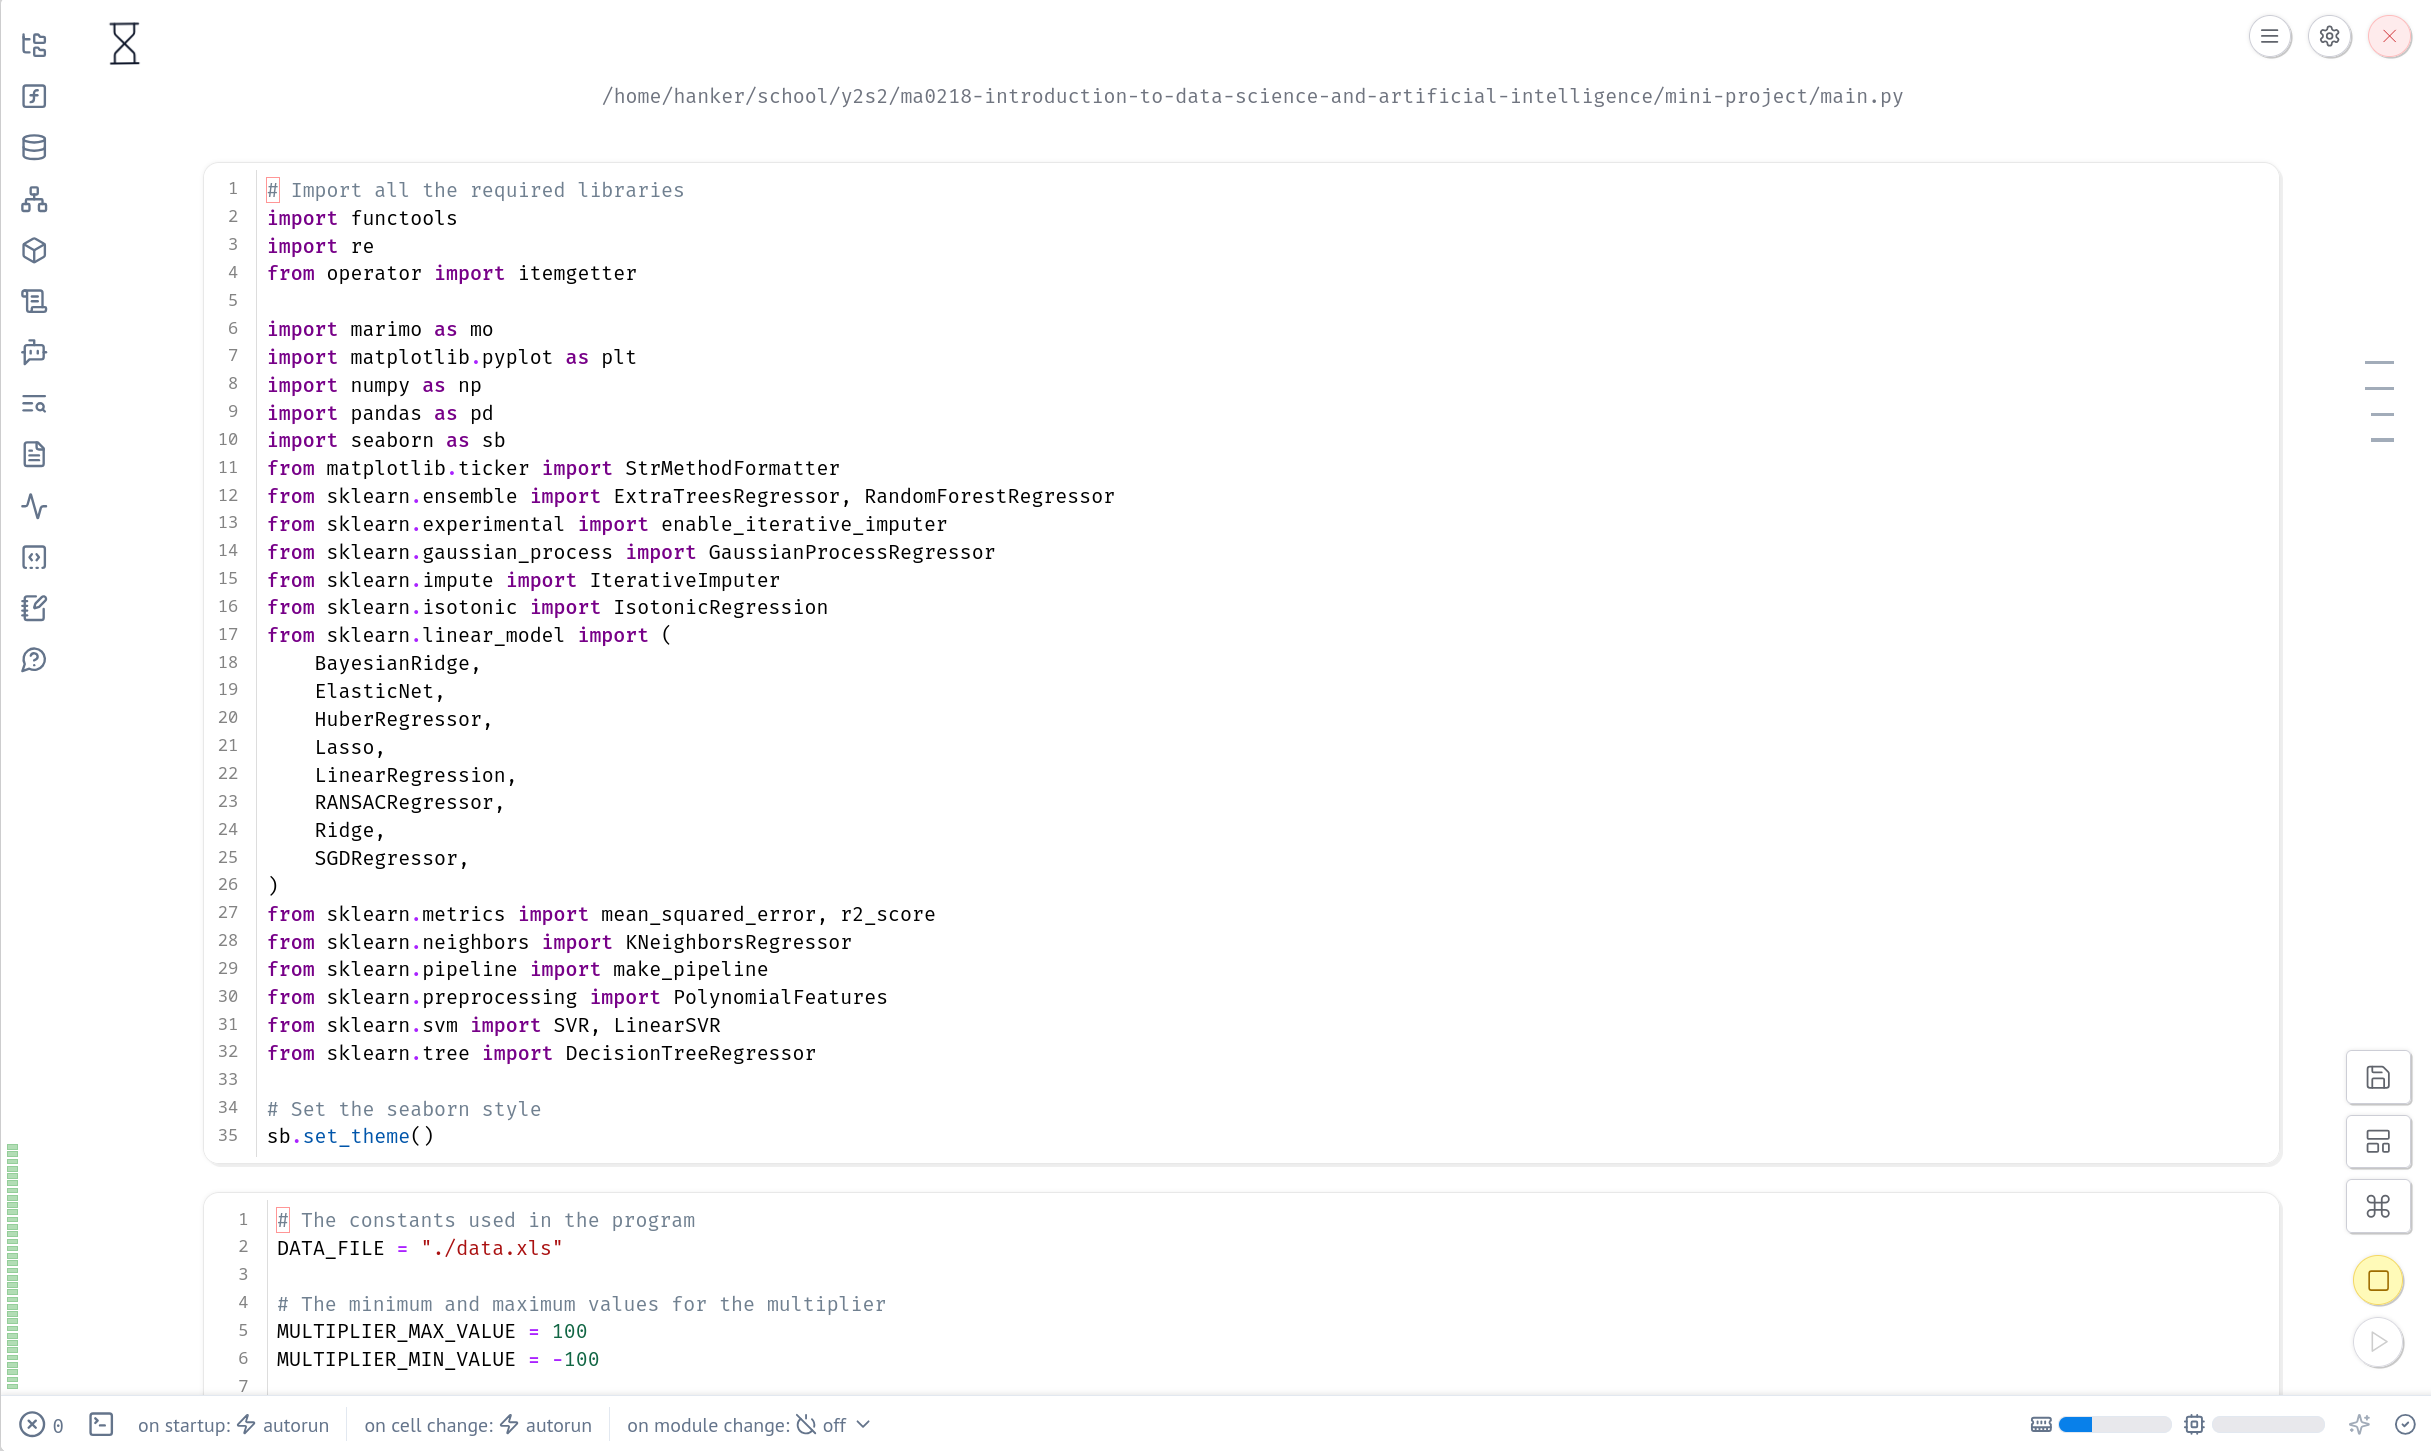
\includegraphics[height=15em]{./images/result-of-editing-the-notebook.png}
\end{center}
\section{Viewing the project without \href{https://marimo.io/}{Marimo}}
\label{sec:org62133e8}

\subsection{Non-interactive notebook using the browser}
\label{sec:org0b9599e}
To view the notebook non-interactively, open the
\href{./notebook.html}{notebook.html} file in your browser.
Double-clicking the file in your file explorer
should be sufficient to view the notebook.
Please be patient, as it takes a while to load.
\subsection{Non-interactive slides using the browser}
\label{sec:orga7ab930}
To view the slides non-interactively, open the
\href{./slides.html}{slides.html} file in your browser.
Double-clicking the file in your file explorer
should be sufficient to view the slides.
Please be patient, as it takes a while to load.
\section{\href{./LICENCE.txt}{Licence}}
\label{sec:org714e7cd}
This project is licensed under the
\href{https://www.gnu.org/licenses/agpl-3.0.en.html}{GNU AGPL v3}.
For the full licence text, you can view the
\href{./LICENCE.txt}{LICENCE.txt} file.
\end{document}
